\chapter{Analysis and Design}
\fancyhead[R]{Analysis and Design}
\label{chap:conception}
\textit{``In this chapter, we dive into the crucial phase of our project, that of analysis and design. This is where abstract aspirations take shape, guided by a deep understanding of needs. This phase is essential for transforming identified requirements into a concrete, structured, and functional solution.''}
\pagebreak

%%%%%%%%%%%%%%%%%%%%%%%%%%%%%%%%%%%%%%%%%%%%%%%%%%%%%%%%%%%%%%%%%%%%%%%%%%%%%%%%%%%%%%%%%%
%%%%%%%%%%%%%%%%%%%%%%%%%%%%%%%%%%%%%%%%%%%%%%%%%%%%%%%%%%%%%%%%%%%%%%%%%%%%%%%%%%%%%%%%%%
%%%%%%%%%%%%%%%%%%%%%%%%%%%%%%%%%%%%%%%%%%%%%%%%%%%%%%%%%%%%%%%%%%%%%%%%%%%%%%%%%%%%%%%%%%
%%%%%%%%%%%%%%%%%%%%%%%%%%%%%%%%%%%%%%%%%%%%%%%%%%%%%%%%%%%%%%%%%%%%%%%%%%%%%%%%%%%%%%%%%%
%%%%%%%%%%%%%%%%%%%%%%%%%%%%%%%%%%%%%%%%%%%%%%%%%%%%%%%%%%%%%%%%%%%%%%%%%%%%%%%%%%%%%%%%%%
%%%%%%%%%%%%%%%%%%%%%%%%%%%%%%%%%%%%%%%%%%%%%%%%%%%%%%%%%%%%%%%%%%%%%%%%%%%%%%%%%%%%%%%%%%

\section{Analysis of the Existing System}

The current P2S compute engine is primarily a monolithic system that processes transactions collectively. It was originally designed to operate with a minimal set of input parameters, which resulted in only medium to low accuracy in fee calculations. Additionally, the system lacks the capability to distribute processing across multiple compute engines, limiting its flexibility and scalability.

To overcome these limitations, the new system is built on a stateless, event-driven architecture that supports enhanced scalability, flexibility, and accuracy where each step is stateless and we can scale on choice the stages of processing that are causing bottlenecks.
 By incorporating multiple specialized compute engines—each handling a specific component of the fee calculation—we aim to create a more modular and efficient framework.

Furthermore, in collaboration with the client, we’ve designed a comprehensive transaction data model that is ISO 20022 compliant and established a shared messaging stream.
 This stream carries a rich set of input parameters (+ 100), enabling the system to consider a wide range of factors in fee calculations and significantly improve result accuracy.


\pagebreak

%%%%%%%%%%%%%%%%%%%%%%%%%%%%%%%%%%%%%%%%%%%%%%%%%%%%%%%%%%%%%%%%%%%%%%%%%%%%%%%%%%%%%%%%%%
%%%%%%%%%%%%%%%%%%%%%%%%%%%%%%%%%%%%%%%%%%%%%%%%%%%%%%%%%%%%%%%%%%%%%%%%%%%%%%%%%%%%%%%%%%
%%%%%%%%%%%%%%%%%%%%%%%%%%%%%%%%%%%%%%%%%%%%%%%%%%%%%%%%%%%%%%%%%%%%%%%%%%%%%%%%%%%%%%%%%%
%%%%%%%%%%%%%%%%%%%%%%%%%%%%%%%%%%%%%%%%%%%%%%%%%%%%%%%%%%%%%%%%%%%%%%%%%%%%%%%%%%%%%%%%%%
%%%%%%%%%%%%%%%%%%%%%%%%%%%%%%%%%%%%%%%%%%%%%%%%%%%%%%%%%%%%%%%%%%%%%%%%%%%%%%%%%%%%%%%%%%



% \subsection{Integration Requirements}

% The system must integrate with:

% \begin{enumerate}
%     \item \textbf{Message Broker Integration}:
%     \begin{itemize}
%         \item Consume transaction messages from Kafka topics
%         \item Publish computed results to designated output topics
%         \item Implement reliable message processing patterns
%     \end{itemize}
    
%     \item \textbf{Database Integration}:
%     \begin{itemize}
%         \item Interact with PostgreSQL for configuration data
%         \item Implement connection pooling for performance
%         \item Support caching for frequently accessed data
%     \end{itemize}
    
%     \item \textbf{Monitoring Integration}:
%     \begin{itemize}
%         \item Provide performance metrics and health checks
%         \item Implement structured logging for troubleshooting
%     \end{itemize}
% \end{enumerate}

% \subsection{Success Criteria}

% The project will be successful when:

% \begin{enumerate}
%     \item \textbf{Functional Completeness}:
%     \begin{itemize}
%         \item All core computation engines are implemented and functional
%         \item Integration with payment processing infrastructure is complete
%         \item Comprehensive validation framework is operational
%     \end{itemize}
    
%     \item \textbf{Performance Achievement}:
%     \begin{itemize}
%         \item System meets required processing performance benchmarks
%         \item Scalability is demonstrated through load testing
%         \item High system availability is maintained
%     \end{itemize}
    
%     \item \textbf{Quality Validation}:
%     \begin{itemize}
%         \item Fee calculation accuracy meets business requirements
%         \item System reliability is validated through testing
%         \item Security and compliance requirements are satisfied
%     \end{itemize}
% \end{enumerate}

% \subsection{Deliverables}

% The project will produce:

% \begin{enumerate}
%     \item \textbf{P2S Compute Engines Implementation}: Production-ready computational framework with all processing engines implemented as scalable microservices.
    
%     \item \textbf{Integration Framework}: Complete message broker and database integration components supporting reliable transaction processing.
    
%     \item \textbf{Validation Framework}: Comprehensive validation system for transaction data and business rule compliance.
    
%     \item \textbf{Technical Documentation}: System architecture documentation including design specifications, integration protocols, and operational procedures.
    
%     \item \textbf{Testing Framework}: Complete testing suite including unit tests, integration tests, and performance validation tools.
% \end{enumerate}




\section{Theoretical Foundation: Event-Driven Architecture}

\subsection{Event-Driven Architecture Principles}

Event-Driven Architecture (EDA) represents a software design paradigm that promotes the production, detection, consumption, and reaction to events \cite{hohpe2003enterprise}. In the context of financial transaction processing, EDA provides several fundamental advantages that address the limitations identified in traditional monolithic architectures.

\subsubsection{Core EDA Concepts}

\textbf{Event Definition and Characteristics:}
An event represents a significant change in state or an occurrence that has business relevance. In payment processing systems, events include transaction initiation, context qualification completion, fee calculation results, and error conditions. Events possess several critical characteristics:

\begin{itemize}
    \item \textbf{Immutability:} Events represent historical facts that cannot be changed
    \item \textbf{Atomicity:} Each event represents a complete, indivisible occurrence
    \item \textbf{Temporal Ordering:} Events carry temporal information enabling proper sequencing
    \item \textbf{Business Relevance:} Each event corresponds to meaningful business activities
\end{itemize}

\textbf{Producer-Consumer Decoupling:}
EDA enables loose coupling between system components through asynchronous message exchange. Event producers generate events without knowledge of consumers, while event consumers process events without direct dependency on producers.

\subsection{EDA Benefits for Financial Processing}

\subsubsection{Scalability and Performance Benefits}

\textbf{Horizontal Scalability:}
EDA enables independent scaling of different processing components based on actual load patterns. Context qualification engines can scale independently from fee calculation engines, optimizing resource utilization and cost efficiency.

\textbf{Asynchronous Processing:}
Non-blocking event processing eliminates wait times and enables higher throughput. Components can process events as resources become available, preventing bottlenecks from cascading through the system.

\subsubsection{Resilience and Fault Tolerance Benefits}

\textbf{Fault Isolation:}
Component failures in EDA systems remain isolated and do not propagate to other components. If the interchange calculation engine fails, context qualification and scheme fee calculation continue operating normally.

\textbf{Automatic Recovery:}
Event persistence in message brokers enables automatic recovery from component failures. When components restart, they can resume processing from their last known position without data loss.

\subsection{Technology Selection Analysis}

\subsubsection{Apache Kafka Selection Rationale}

Apache Kafka was selected as the message broker for the P2S compute engines based on comprehensive technology analysis:

\begin{table}[h]
\centering
\begin{tabular}{|l|c|c|c|c|}
\hline
\textbf{Technology} & \textbf{Throughput} & \textbf{Durability} & \textbf{Scalability} & \textbf{Financial Suitability} \\
\hline
Apache Kafka & High & High & High & Excellent \\
RabbitMQ & Medium & Medium & Medium & Good \\
Amazon SQS & Medium & High & High & Good \\
Apache Pulsar & High & High & High & Good \\
\hline
\end{tabular}
\caption{Message Broker Technology Comparison}
\end{table}

\textbf{Kafka Advantages for Fee Calculation:}
\begin{itemize}
    \item \textbf{Exactly-Once Semantics:} Critical for financial accuracy requirements
    \item \textbf{High Throughput:} Supports millions of transactions per second
    \item \textbf{Event Replay:} Enables transaction replay for testing and audit
    \item \textbf{Stream Processing:} Native support for real-time analytics
\end{itemize}

\section{Solution Architecture Design}

\subsection{Microservices Architecture Selection}

The adoption of microservices architecture for the P2S compute engines addresses the fundamental limitations of the existing monolithic system while providing specific advantages for financial transaction processing.

\subsubsection{Domain-Driven Design Alignment}

Each microservice aligns with specific business domains:
\begin{itemize}
    \item \textbf{Meta Worker:} Transaction routing and enrichment domain
    \item \textbf{Context Engine:} Transaction qualification and categorization domain
    \item \textbf{Interchange Engine:} Bilateral fee calculation domain
    \item \textbf{Scheme Fee Engine:} Network-specific fee calculation domain
\end{itemize}

\subsubsection{Stateless Processing Design}

All P2S compute engines implement stateless processing patterns where each request contains complete information necessary for processing. This design provides:

\begin{itemize}
    \item \textbf{Linear Scalability:} New instances can be added without state synchronization
    \item \textbf{Fault Recovery:} Component restart does not require state restoration
    \item \textbf{Load Distribution:} Requests can be processed by any available instance
    \item \textbf{Simplified Testing:} Each request can be tested independently
\end{itemize}

\section{System Design and UML Modeling}

\subsection{Class Diagram Analysis}

The UML class diagram provides a visual representation of the system's classes, their attributes, methods, and relationships. It serves as a blueprint for the stateless compute engine implementation and illustrates the architectural foundations of the event-driven system.

In the P2S Compute Engines system, the class diagram demonstrates several key architectural patterns:

\begin{figure}[H]
    \centering
    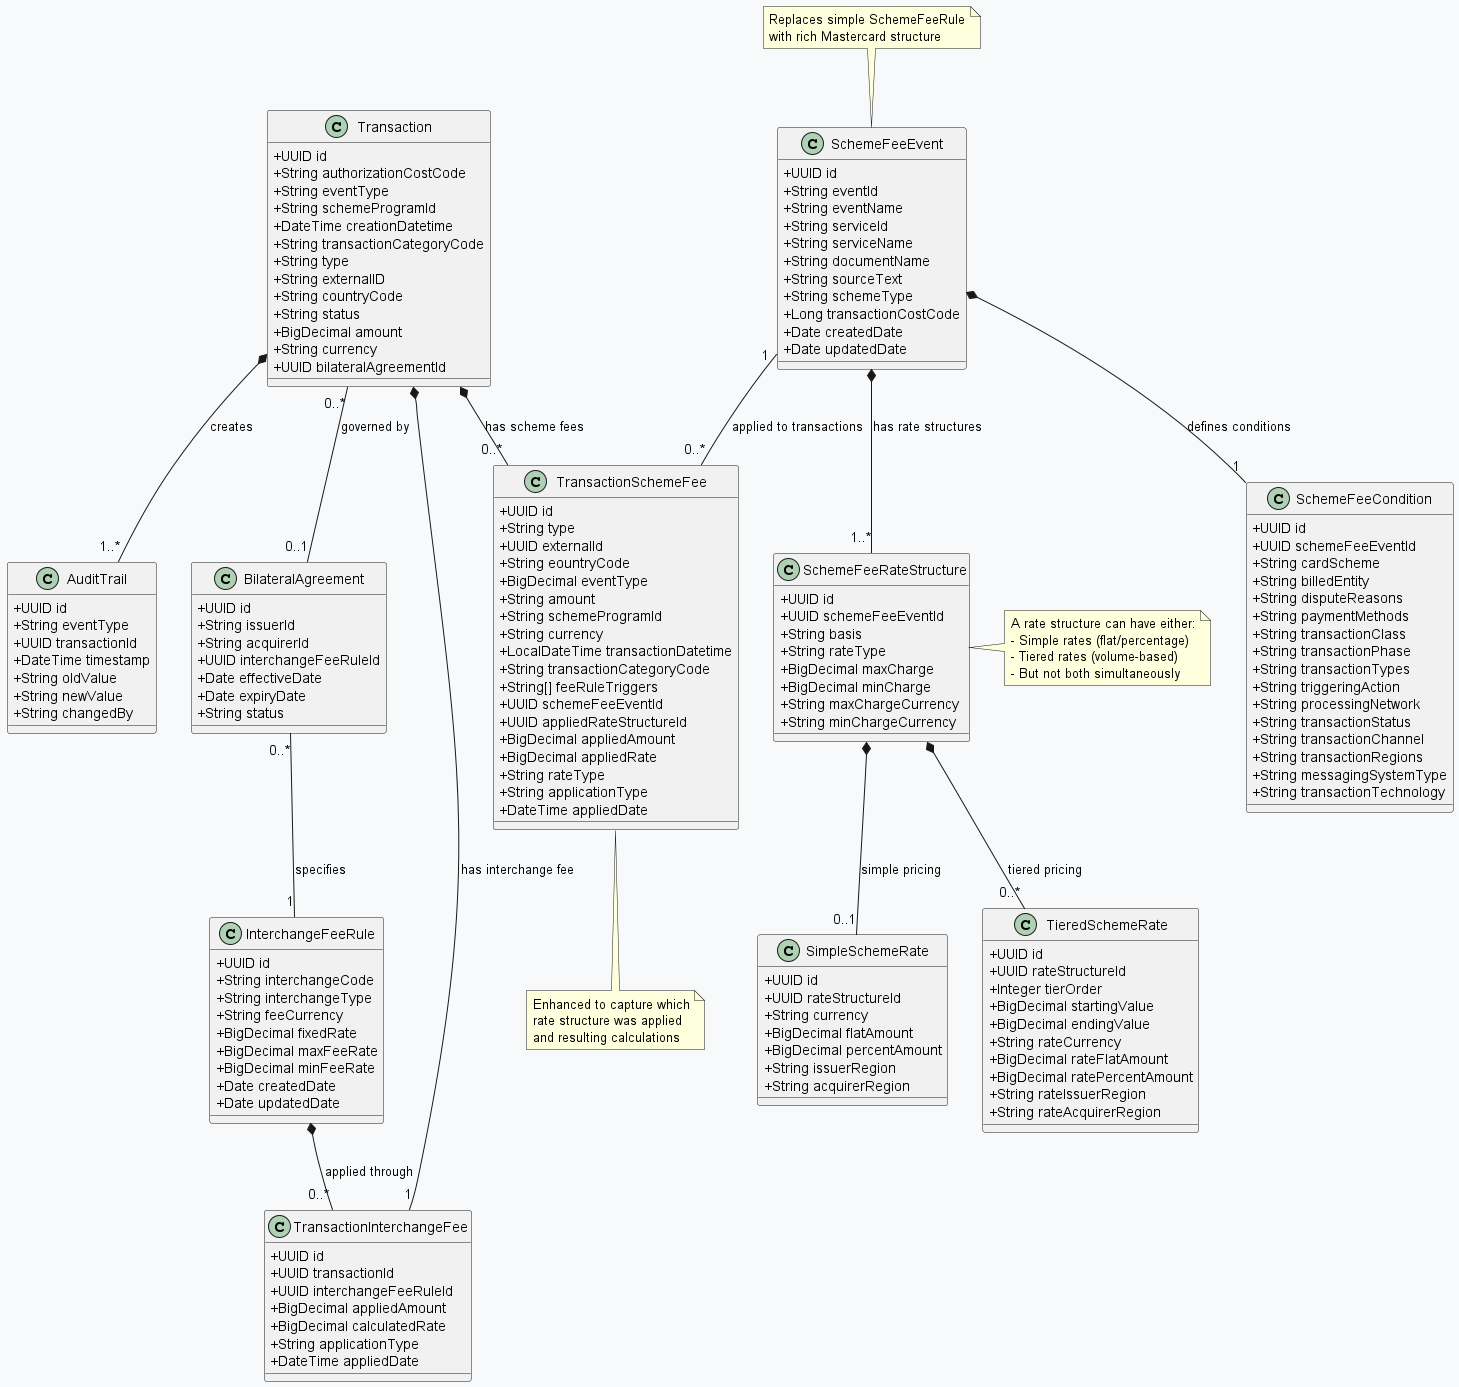
\includegraphics[width=1.05\textwidth]{out/diagrams/plantuml/in/class-diagram/class-diagram.png}
    \caption{UML Class Diagram for P2S Compute Engines}
    \label{fig:class_diagram}
\end{figure}

\subsubsection{Class Diagram Analysis}

The class diagram illustrates the core architectural components and their relationships within the P2S compute engines:

\textbf{Worker Engine Hierarchy:}
The diagram shows a clear hierarchy of worker engines, each implementing specialized processing logic:
\begin{itemize}
    \item \textbf{BaseWorkerEngine:} Abstract base class providing common functionality for message processing, error handling, and lifecycle management
    \item \textbf{MetaWorkerEngine:} Extends base functionality to provide transaction enrichment and routing capabilities
    \item \textbf{ContextQualificationEngine:} Implements business rule evaluation for transaction categorization
    \item \textbf{InterchangeCalculationEngine:} Specializes in bilateral fee calculation algorithms
    \item \textbf{SchemeFeeCalculationEngine:} Handles network-specific fee computation logic
\end{itemize}

\textbf{Data Model Classes:}
The diagram demonstrates the rich data model supporting 100+ transaction parameters:
\begin{itemize}
    \item \textbf{TransactionMessage:} Core transaction data structure containing ISO 20022 compliant fields
    \item \textbf{ProcessingContext:} Enrichment data added during processing stages
    \item \textbf{FeeCalculationResult:} Standardized result structure for fee computation outputs
    \item \textbf{ErrorContext:} Comprehensive error information for debugging and audit
\end{itemize}

\textbf{Integration Components:}
The class relationships show clear separation of concerns for external system integration:
\begin{itemize}
    \item \textbf{KafkaMessageHandler:} Manages event consumption and production
    \item \textbf{DatabaseAccessLayer:} Provides abstraction for PostgreSQL operations
    \item \textbf{CacheManager:} Handles Redis cache operations and invalidation
    \item \textbf{ConfigurationManager:} Manages system configuration and fee rules
\end{itemize}



\subsection{Use Case Diagram Analysis}

The use case diagram provides a visual representation of the interactions between actors and the system, highlighting the key functionalities and their relationships. It demonstrates how different stakeholders interact with the P2S compute engines and the value provided by each interaction.

\begin{figure}[H]
    \centering
    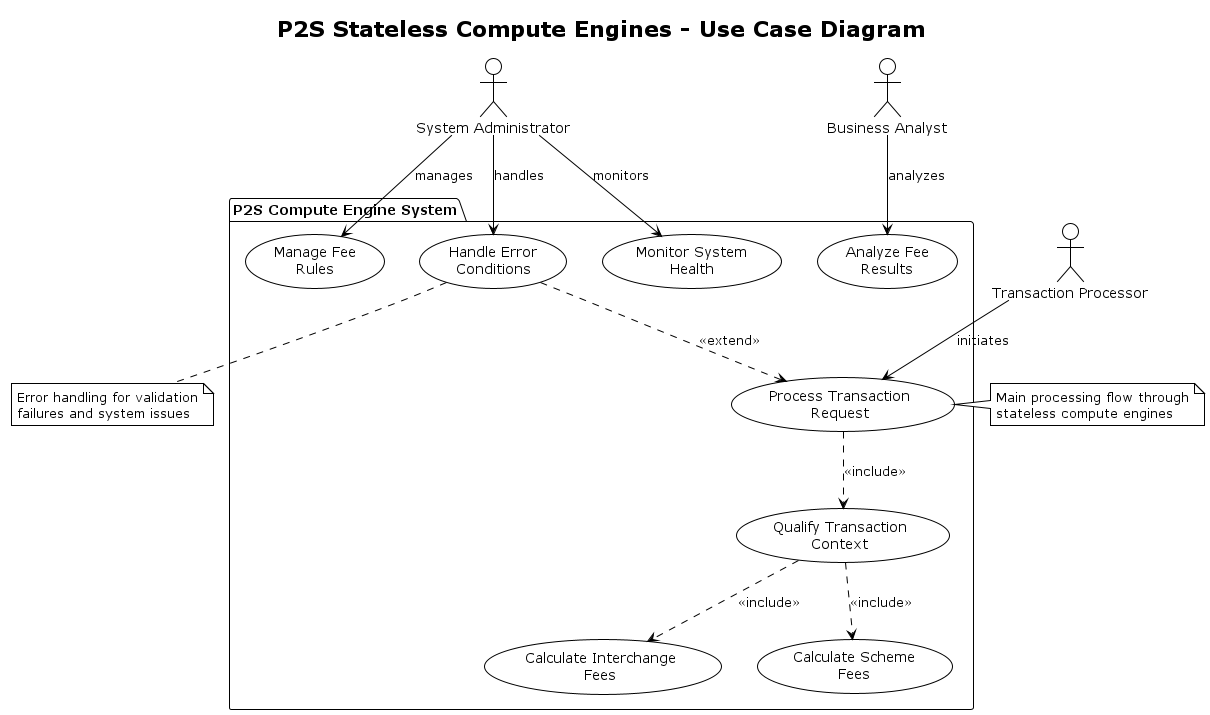
\includegraphics[width=1.05\textwidth]{out/diagrams/plantuml/in/use-case/use-case.png}
    \caption{Use Case Diagram for P2S Compute Engines}
    \label{fig:use_case_diagram}
\end{figure}

\subsubsection{Actor and Use Case Analysis}

The use case diagram identifies key actors and their interactions:

\textbf{Primary Actors:}
\begin{itemize}
    \item \textbf{Transaction Processor:} Submits raw transaction data for fee calculation
    \item \textbf{System Administrator:} Manages system configuration and monitoring
    \item \textbf{Business Analyst:} Analyzes fee calculation results and validates business rules
\end{itemize}

\textbf{Core Use Cases:}
\begin{itemize}
    \item \textbf{Process Transaction:} End-to-end transaction processing through fee calculation pipeline
    \item \textbf{Calculate Interchange Fees:} Bilateral fee computation between banks
    \item \textbf{Calculate Scheme Fees:} Network-specific fee calculation
    \item \textbf{Qualify Transaction Context:} Business rule evaluation and categorization
    \item \textbf{Monitor System Health:} Real-time performance and operational monitoring
\end{itemize}

\subsection{Sequence Diagram Analysis}

The sequence diagrams illustrate the detailed flow of interactions between components during transaction processing scenarios. They demonstrate the event-driven communication patterns and the temporal ordering of processing activities across the distributed system architecture.

\subsubsection{Context Qualification Sequence Diagram}

The context qualification sequence diagram demonstrates the sophisticated business rule evaluation process that categorizes transactions based on multiple contextual factors.

\begin{figure}[H]
    \centering
    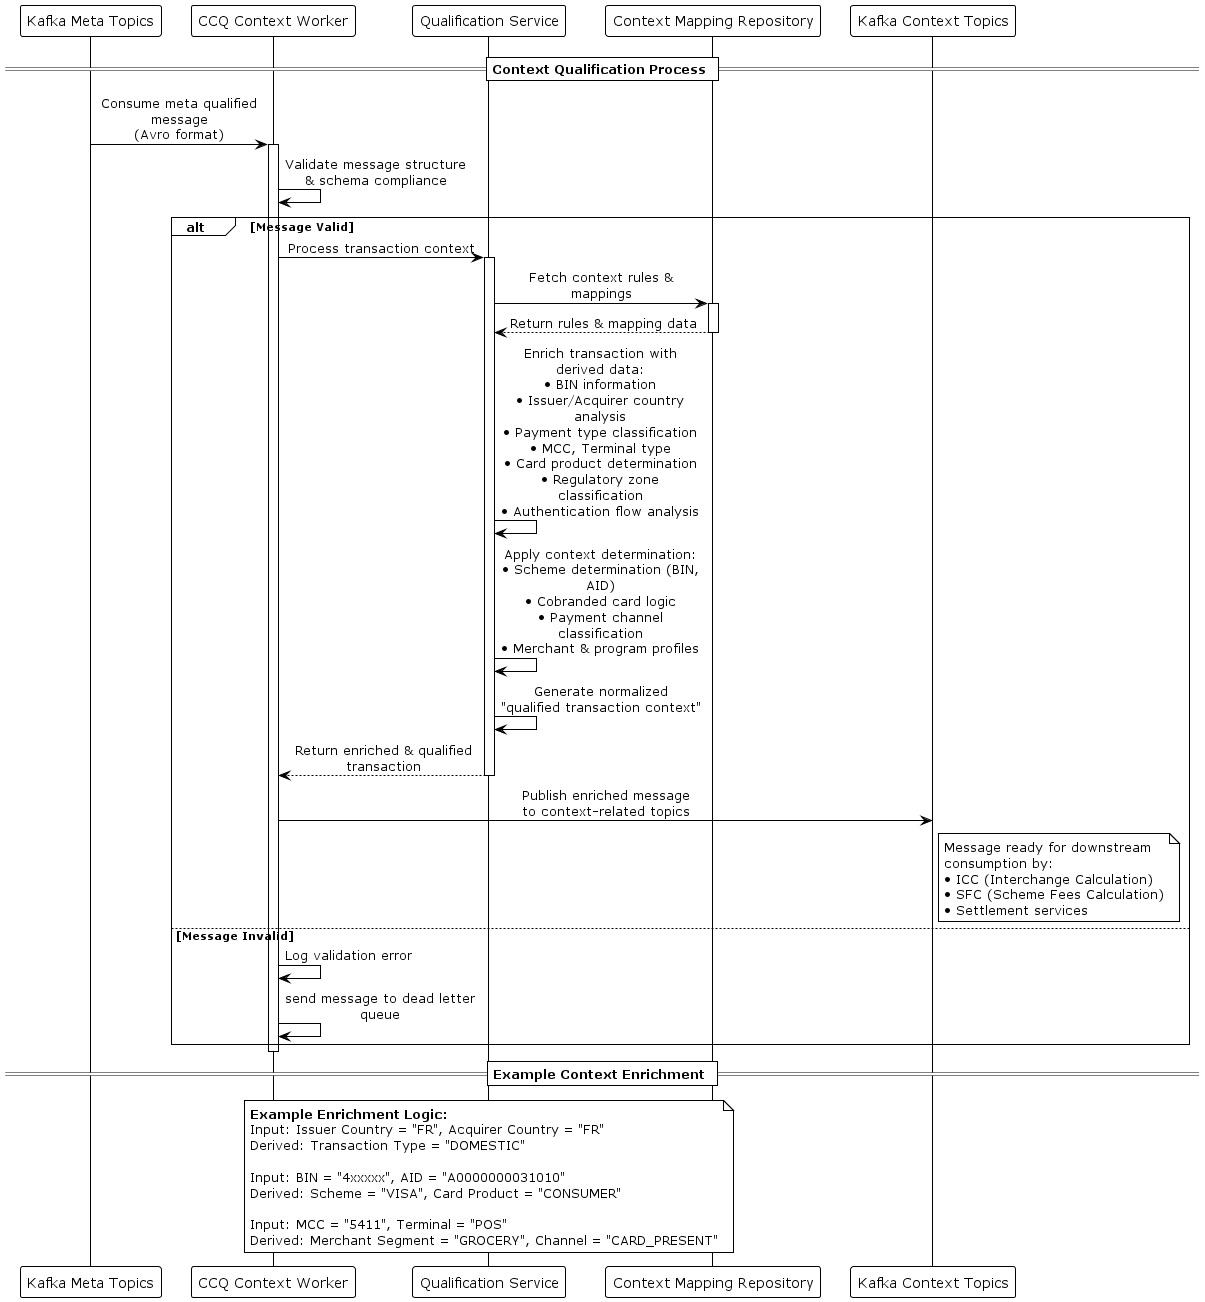
\includegraphics[width=1.05\textwidth]{out/diagrams/plantuml/in/context-sequence-diagram/P2S Context Qualification Process.png}
    \caption{Context Qualification Sequence Diagram}
    \label{fig:context_qualification_sequence}
\end{figure}   

\textbf{Process Flow Analysis:}
The sequence diagram illustrates the following key processing steps:

\begin{enumerate}
    \item \textbf{Message Consumption:} Context engine consumes enriched transaction from meta-output topic
    \item \textbf{Rule Retrieval:} Engine queries database for applicable business rules based on transaction characteristics
    \item \textbf{Cache Optimization:} Frequently used rules retrieved from Redis cache to minimize database load
    \item \textbf{Context Evaluation:} Multiple contextual factors evaluated including geography, merchant category, card product type
    \item \textbf{Qualification Decision:} Business rules applied to determine transaction qualification category
    \item \textbf{Result Publication:} Qualified transaction published to p2s-context-out topic for downstream processing
    \item \textbf{Error Handling:} Processing errors captured and routed to dedicated error topic
\end{enumerate}

\textbf{Design Patterns Demonstrated:}
\begin{itemize}
    \item \textbf{Event-Driven Processing:} Asynchronous message consumption and production
    \item \textbf{Cache-Aside Pattern:} Database queries with cache fallback for performance optimization
    \item \textbf{Dead Letter Queue:} Error isolation and retry mechanism implementation
    \item \textbf{Correlation ID Tracking:} End-to-end transaction tracing for observability
\end{itemize}

\subsubsection{Interchange Calculation Sequence Diagram}

The interchange calculation sequence diagram shows the complex bilateral fee computation process between issuing and acquiring banks.

\begin{figure}[H]
    \centering
    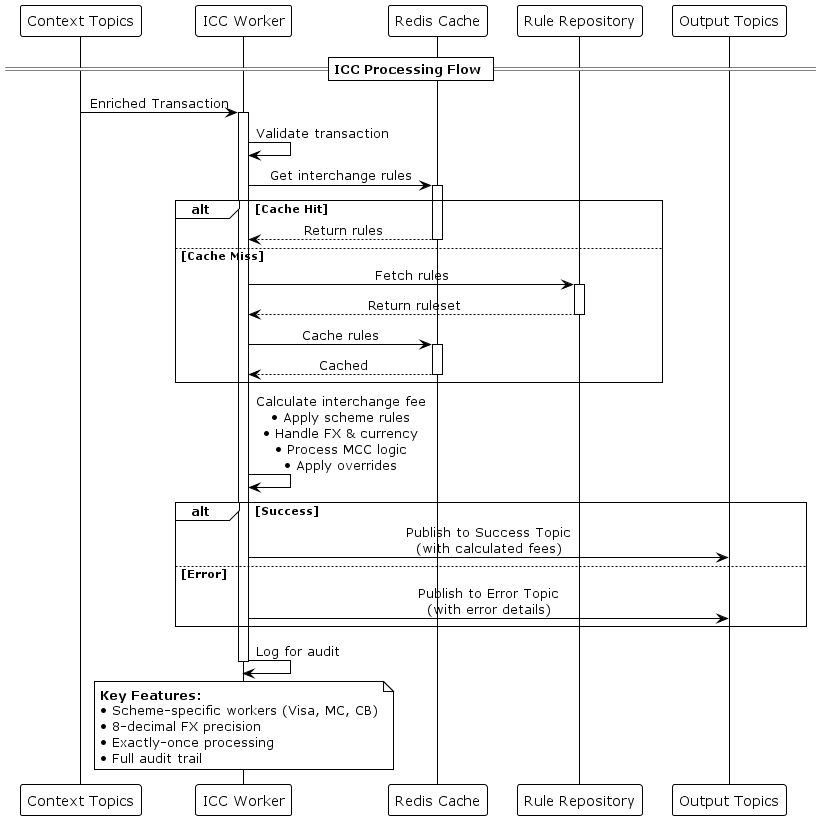
\includegraphics[width=1.05\textwidth]{out/diagrams/plantuml/in/ic-sequence/P2S Interchange Fee Calculation Process.png}
    \caption{Interchange Calculation Sequence Diagram}
    \label{fig:interchange_calculation_sequence}
\end{figure}

\textbf{Process Flow Analysis:}
The interchange calculation process demonstrates sophisticated fee computation logic:

\begin{enumerate}
    \item \textbf{Qualified Transaction Input:} Engine consumes qualified transactions from context output topic
    \item \textbf{Bilateral Agreement Lookup:} System queries for specific agreements between issuer and acquirer
    \item \textbf{Regulatory Compliance Check:} Verification of fee caps and regulatory constraints
    \item \textbf{Multi-Dimensional Calculation:} Fee computation based on transaction amount, geography, card type, and merchant category
    \item \textbf{Currency Conversion:} Cross-border transaction handling with appropriate exchange rates
    \item \textbf{Result Validation:} Calculated fees validated against business rules and regulatory limits
    \item \textbf{Publication:} Results published to interchange output topic for consolidation
\end{enumerate}

\textbf{Financial Processing Patterns:}
\begin{itemize}
    \item \textbf{Multi-Factor Fee Calculation:} Complex algorithm considering multiple transaction attributes
    \item \textbf{Regulatory Compliance:} Automated validation against interchange fee regulations
    \item \textbf{Bilateral Agreement Processing:} Priority-based rule application for bank-specific agreements
    \item \textbf{Audit Trail Generation:} Comprehensive logging for regulatory compliance and debugging
\end{itemize}

\subsubsection{Scheme Fees Calculation Sequence Diagram}

The scheme fees calculation sequence diagram illustrates network-specific fee computation for payment scheme operations.

\begin{figure}[H]
    \centering
    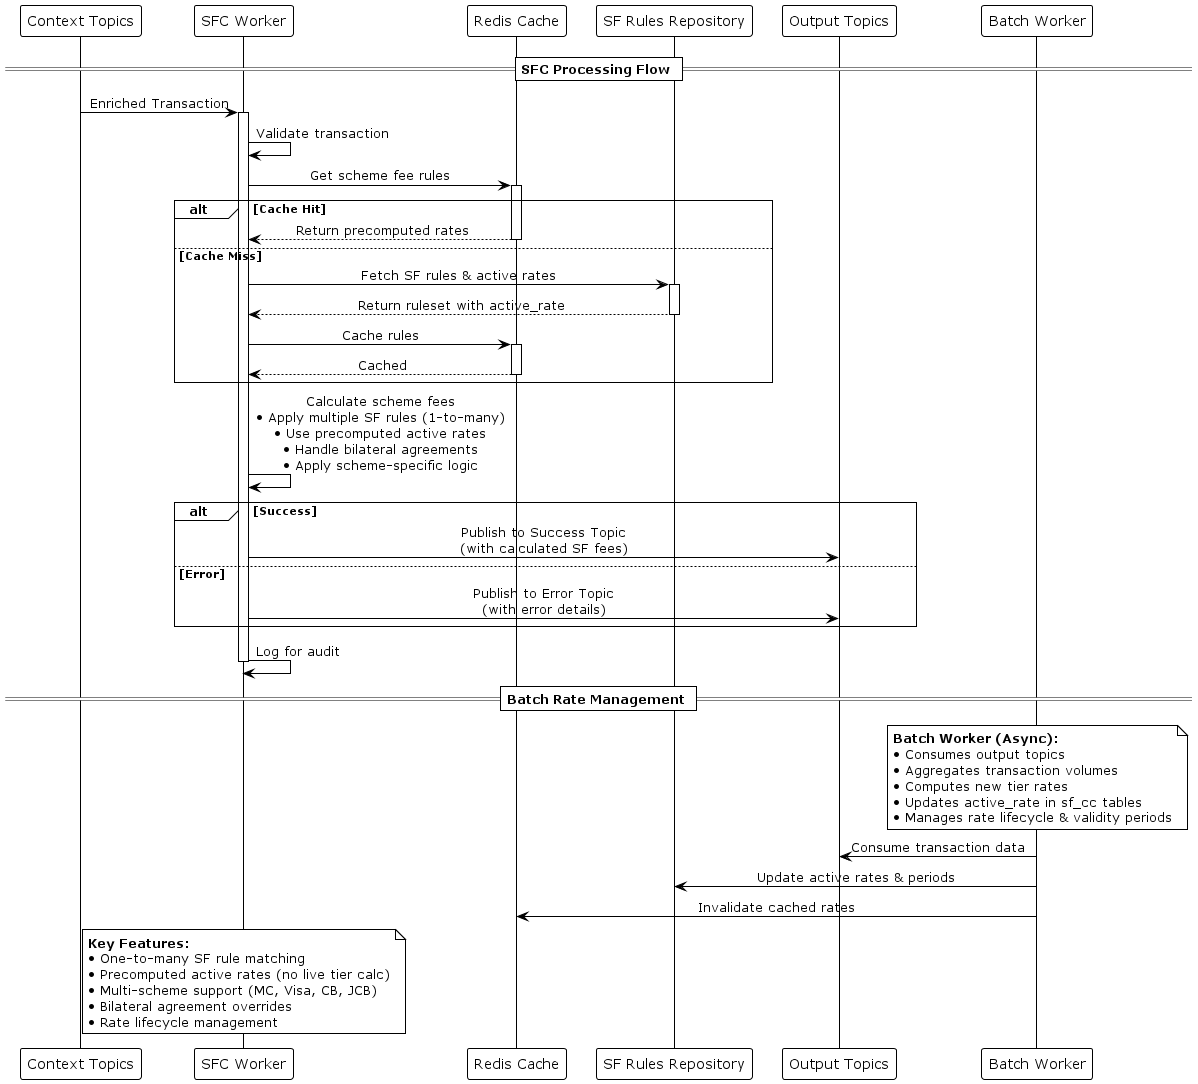
\includegraphics[width=1.05\textwidth]{out/diagrams/plantuml/in/sf-sequence/P2S Scheme Fee Calculation Process.png}
    \caption{Scheme Fees Calculation Sequence Diagram}
    \label{fig:scheme_fees_calculation_sequence}
\end{figure}

\textbf{Process Flow Analysis:}
The scheme fee calculation process demonstrates network-specific fee logic:

\begin{enumerate}
    \item \textbf{Transaction Consumption:} Engine processes qualified transactions from context output
    \item \textbf{Scheme Identification:} Payment network identification (Visa, Mastercard) for appropriate fee structure
    \item \textbf{Cost Code Resolution:} Hierarchical cost code determination based on transaction attributes
    \item \textbf{Volume Threshold Analysis:} Institution-specific volume thresholds for progressive pricing
    \item \textbf{Service Fee Calculation:} Specialized fees for premium services and enhanced processing
    \item \textbf{Promotional Rate Application:} Time-based promotional rates and discount application
    \item \textbf{Result Aggregation:} Multiple fee components combined into final scheme fee amount
\end{enumerate}

\textbf{Network Processing Patterns:}
\begin{itemize}
    \item \textbf{Hierarchical Cost Codes:} Multi-level fee categorization based on transaction characteristics
    \item \textbf{Volume-Based Pricing:} Progressive fee structures based on institutional transaction volumes
    \item \textbf{Temporal Fee Variations:} Time-sensitive promotional rates and special pricing
    \item \textbf{Network-Specific Logic:} Specialized algorithms for different payment scheme methodologies
\end{itemize}

\subsection{Design Pattern Integration}

The sequence diagrams collectively demonstrate the integration of several important design patterns within the P2S compute engines:

\textbf{Event-Driven Patterns:}
\begin{itemize}
    \item \textbf{Publish-Subscribe:} Kafka topics enable loose coupling between processing stages
    \item \textbf{Event Sourcing:} Complete transaction processing history maintained through event sequence
    \item \textbf{CQRS:} Separation of command (processing) and query (monitoring) responsibilities
\end{itemize}

\textbf{Resilience Patterns:}
\begin{itemize}
    \item \textbf{Circuit Breaker:} Prevents cascade failures during database or cache outages
    \item \textbf{Retry Pattern:} Automatic retry with exponential backoff for transient failures
    \item \textbf{Bulkhead:} Error isolation through dedicated error topics and processing lanes
\end{itemize}

\textbf{Performance Patterns:}
\begin{itemize}
    \item \textbf{Cache-Aside:} Redis caching with database fallback for optimal performance
    \item \textbf{Connection Pooling:} Efficient database connection management
    \item \textbf{Asynchronous Processing:} Non-blocking operations for maximum throughput
\end{itemize}

%%%%%%%%%%%%%%%%%%%%%%%%%%%%%%%%%%%%%%%%%%%%%%%%%%%%%%%%%%%%%%%%%%%%%%%%%%%%%%%%%%%%%%%%%%
%%%%%%%%%%%%%%%%%%%%%%%%%%%%%%%%%%%%%%%%%%%%%%%%%%%%%%%%%%%%%%%%%%%%%%%%%%%%%%%%%%%%%%%%%%
%%%%%%%%%%%%%%%%%%%%%%%%%%%%%%%%%%%%%%%%%%%%%%%%%%%%%%%%%%%%%%%%%%%%%%%%%%%%%%%%%%%%%%%%%%
%%%%%%%%%%%%%%%%%%%%%%%%%%%%%%%%%%%%%%%%%%%%%%%%%%%%%%%%%%%%%%%%%%%%%%%%%%%%%%%%%%%%%%%%%%
%%%%%%%%%%%%%%%%%%%%%%%%%%%%%%%%%%%%%%%%%%%%%%%%%%%%%%%%%%%%%%%%%%%%%%%%%%%%%%%%%%%%%%%%%%
%%%%%%%%%%%%%%%%%%%%%%%%%%%%%%%%%%%%%%%%%%%%%%%%%%%%%%%%%%%%%%%%%%%%%%%%%%%%%%%%%%%%%%%%%%

%%%%%%%%%%%%%%%%%%%%%%%%%%%%%%%%%%%%%%%%%%%%%%%%%%%%%%%%%%%%%%%%%%%%%%%%%%%%%%%%%%%%%%%%%%
%%%%%%%%%%%%%%%%%%%%%%%%%%%%%%%%%%%%%%%%%%%%%%%%%%%%%%%%%%%%%%%%%%%%%%%%%%%%%%%%%%%%%%%%%%
%%%%%%%%%%%%%%%%%%%%%%%%%%%%%%%%%%%%%%%%%%%%%%%%%%%%%%%%%%%%%%%%%%%%%%%%%%%%%%%%%%%%%%%%%%
%%%%%%%%%%%%%%%%%%%%%%%%%%%%%%%%%%%%%%%%%%%%%%%%%%%%%%%%%%%%%%%%%%%%%%%%%%%%%%%%%%%%%%%%%%
%%%%%%%%%%%%%%%%%%%%%%%%%%%%%%%%%%%%%%%%%%%%%%%%%%%%%%%%%%%%%%%%%%%%%%%%%%%%%%%%%%%%%%%%%%
%%%%%%%%%%%%%%%%%%%%%%%%%%%%%%%%%%%%%%%%%%%%%%%%%%%%%%%%%%%%%%%%%%%%%%%%%%%%%%%%%%%%%%%%%%

\section{Architecture Design Summary}

\subsection{Design Decision Validation}

The comprehensive analysis presented in this chapter validates the key architectural decisions made for the P2S compute engines proof-of-concept implementation:

\textbf{Event-Driven Architecture Selection:}
The theoretical analysis and practical implementation demonstrate that event-driven architecture provides the optimal foundation for financial transaction processing systems requiring high throughput, fault tolerance, and scalability. The benefits of producer-consumer decoupling, automatic recovery, and horizontal scalability directly address the limitations identified in traditional monolithic approaches.

\textbf{Microservices Decomposition:}
The domain-driven decomposition into specialized engines (Meta, Context, Interchange, Scheme Fee) enables independent optimization, scaling, and evolution of each processing concern. This approach provides the flexibility necessary for adapting to changing business requirements and payment scheme updates.

\textbf{Stateless Processing Design:}
The stateless processing pattern eliminates complex state management requirements while enabling linear horizontal scaling. The externalization of state through databases and caching layers provides the performance benefits of stateless processing while maintaining necessary data persistence.

\subsection{Technology Integration Analysis}

The technology selection analysis validates the chosen technology stack for financial processing requirements:

\textbf{Apache Kafka Integration:}
Kafka's exactly-once semantics, high throughput capabilities, and event replay functionality provide the reliability and performance characteristics required for financial transaction processing \cite{narkhede2017kafka}. The comprehensive comparison with alternative technologies confirms Kafka as the optimal choice for the P2S platform.

\textbf{Database and Caching Strategy:}
The combination of PostgreSQL for transactional data and Redis for caching provides optimal balance between data consistency, performance, and operational complexity. The cache-aside pattern implementation demonstrates effective performance optimization without compromising data integrity.

\subsection{UML Model Insights}

The UML modeling analysis provides several critical insights into the system design:

\textbf{Class Structure Validation:}
The class diagram demonstrates clear separation of concerns between processing logic, data management, and system integration. The inheritance hierarchy for worker engines provides code reuse while enabling specialized optimization for different fee calculation types.

\textbf{Use Case Coverage:}
The use case analysis confirms that the system design addresses all critical stakeholder requirements, from transaction processing to system administration and monitoring. The identified actor relationships validate the system's integration points with external systems and personnel.

\textbf{Sequence Flow Optimization:}
The detailed sequence diagram analysis reveals optimized processing flows that minimize latency while maintaining comprehensive error handling and audit trail generation. The event-driven communication patterns enable parallel processing where appropriate while preserving necessary sequencing for dependent operations.

\subsection{Design Pattern Implementation}

The architecture successfully integrates multiple design patterns that collectively address the complex requirements of financial transaction processing:

\textbf{Scalability Patterns:}
The implementation of event-driven, stateless, and microservices patterns creates a foundation for linear horizontal scaling that can adapt to varying transaction volumes and processing requirements.

\textbf{Resilience Patterns:}
Circuit breakers, retry mechanisms, and bulkhead isolation patterns ensure system resilience during failure conditions while maintaining processing continuity for unaffected components.

\textbf{Performance Patterns:}
Caching, connection pooling, and asynchronous processing patterns optimize system performance while maintaining the accuracy and reliability requirements of financial processing.

\section{Chapter Conclusion}

This chapter has established the comprehensive theoretical and practical foundation for the P2S compute engines architecture. The analysis demonstrates how event-driven architecture principles address the fundamental limitations of traditional monolithic payment processing systems while providing the scalability, resilience, and performance characteristics required for modern financial transaction processing.

The detailed examination of technology selection criteria validates the chosen technology stack as optimal for the specific requirements of fee calculation systems. The comprehensive UML analysis provides both high-level architectural understanding and detailed implementation guidance for the subsequent development phases.

The integration of proven design patterns throughout the architecture ensures that the system can meet both current proof-of-concept objectives and future production-scale requirements. The stateless, event-driven approach provides the foundation for the horizontal scaling and operational excellence necessary for enterprise financial processing environments.

\textbf{Key Architectural Achievements:}
\begin{itemize}
    \item \textbf{Scalability Foundation:} Event-driven, stateless architecture enabling linear horizontal scaling
    \item \textbf{Resilience Framework:} Comprehensive error handling and recovery mechanisms
    \item \textbf{Performance Optimization:} Multi-tier caching and asynchronous processing patterns
    \item \textbf{Business Alignment:} Domain-driven microservices aligned with financial processing requirements
    \item \textbf{Technology Integration:} Validated technology stack optimized for financial processing needs
\end{itemize}

The next chapter will demonstrate how these architectural principles translate into practical implementation, validating the theoretical foundation through concrete proof-of-concept development and performance testing.